\title{The brown recluse spider (\textit{Loxosceles reclusa}) continues to not occur in Alaska and no specimens from Alaska have ever been archived}

\subtitle{\doi{10.----------}}

\author{by Derek S.\ Sikes\footnote{University of Alaska Museum, Fairbanks, AK, USA}}

\maketitle

A species notably absent from the Alaskan arthropod fauna and worth commenting on is a spider often found indoors in its native range, \textit{Loxosceles reclusa} Gertsch \& Mulaik, 1940  (brown recluse spider). No scientific records of this species exist for Alaska \citep{Simpsonetal2019} despite the belief by some residents of the state that this spider has been present or may even maintain breeding populations in the state. This spider is a well-known species of medical concern and considerable confusion exists in the general public concerning its geographic distribution and habits \citep{VetterBush2002}. 

Over the past decade, many specimens and photographs of spiders have been submitted to staff of the University of Alaska Museum (\acr{UAM}) Insect Collection by people who suspected they had found this species in Alaska, but none were the brown recluse. This is not surprising, since this spider is rarely found outside of its native range in the midwest and southcentral \acr{US} states (Figure \ref{recluse_map}) \citep{VetterBush2002, GBIF2020, iNaturalist2020}. 

The spider fauna of Alaska includes over 620 species and the University of Alaska Museum Insect Collection has over 43,000 Alaskan archived spider specimens \citep{Sikesetal2017}, making spiders one of the more well documented arthropod groups for the state. Although it is sometimes said that, ``absence of evidence is not evidence of absence,'' all evidence to date, combined with the known ecology of this species, indicates it does not occur in Alaska. The University of Alaska Museum Insect Collection is happy to receive specimens or photographs of spiders found in Alaska thought to be the brown recluse. A population must be found in Alaska and specimens archived before this species can be officially considered present in the state. Reports of bites, medical diagnoses, and sightings without specimens are insufficient because many injuries are mistakenly diagnosed as spider bites \citep{VetterBush2002} and the spider cannot be identified with confidence without preserved specimens under a microscope or high-quality macrophotographic images.

However, it is possible this species could establish indoors in Alaska. Shipments of goods from within its native range to Alaska and the effects of climate change all increase the chances of it being found in Alaska someday. A close relative from Chile, \textit{Loxosceles laeta} (Nicolet, 1849), has been living non-captive in the Finnish Museum of Natural History in Helsinki since it was introduced in 1963 \citep{Huhta1972, Nicholls2016}. Despite almost 60 years during which this medically important spider has had free reign within the Helsinki museum, only one bite has been recorded, and there was no lasting damage \citep{Nicholls2016}.

In contrast to the absence of specimens of recluse spiders in Alaska, non-native \textit{Latrodectus} spp. (widow spiders), have been found in Alaska in shipments from lower latitude states. None have ever established a breeding population, however. A summary of known interceptions of these spiders in Alaska can be found in \citet{Bowser2013}. An adult female \textit{Latrodectus hesperus} was kept in captivity inside \acr{UAM} as part of an educational display in 2012 called ``Leggy!'' \citep{Sikes2012} but was killed when the exhibit ended.

\section{Acknowledgments}
I thank Yuri Marusik for telling me about the Helsinki population of \textit{L.\ laeta.}

\bibliography{recluse}

\end{multicols}
\begin{figure}[H]
\begin{center}
%\vspace{2mm}
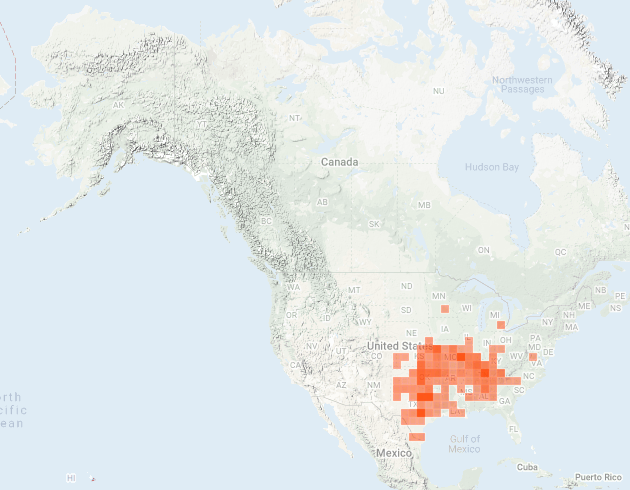
\includegraphics[width=15cm]{img/recluse.png}
\caption{Research-grade iNaturalist observation records ($n=764$) of \textit{Loxosceles reclusa} as of 26 March 2020 \citep{iNaturalist2020}.}
\label{recluse_map}
\end{center}
\end{figure} 
\begin{multicols}{2} 
